\documentclass[a4paper]{report}
\usepackage[utf8]{inputenc}
\usepackage[T1]{fontenc} 
\usepackage[francais]{babel}
\usepackage{graphicx}
\usepackage{geometry}
\usepackage{color}
\usepackage{fancyhdr}
\pagestyle{fancy}
\fancyhf{}
\lhead{2011/2012}
\rhead{IUT Nancy Charlemagne}
\geometry{hmargin=1cm,vmargin=2cm,lmargin=2cm,rmargin=2cm}
\lfoot{Mathieu LEROUX}
\cfoot{Rapport intemédiaire (compression,déduplication et ZFS) \\ Licence ASRALL}
\rfoot{\thepage}
\renewcommand{\footrulewidth}{2pt}
\begin{document}
	\chapter*{Déduplication}
	La déduplication de données est une technique qui permet de minimiser de l'espace de stockage. Elle consiste à ne pas répliquer les données déja existantes sur le disque. Un fichier est décomposé sous forme de blocs de données car des fichiers peuvent avoir des blocs en commum. Le mécanisme de déduplication crée une table avec les index de tous les blocs de données des fichiers présents sur le disque. La taille des blocs peut varier selon les mécanismes utilisés mais plus les blocs sont petits, plus il y aura de chance qu'un autre bloc soit identique et donc, plus la déduplication sera efficace. En général, cette taille ne dépasse pas les 128ko.
 
 Quand un utilisateur dépose un fichier, le mécanisme crée ses index et regarde s'il n'y a pas des blocs déjà existants. Si des blocs sont similaires alors une simple référence aux blocs déjà existants sera crée. Le schéma ci-dessous montre comment la déduplication fonctionne. Les blocs étant de la même couleur sont considérés identiques.\\
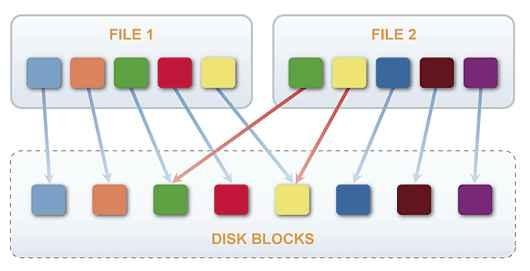
\includegraphics[width=10cm]{deduplication.jpg}

Il existe deux types de dépuplication: la déduplication à la volée (à la source) et la déduplication hors ligne (à la destination). La déduplication à la volée analyse les fichiers avant de les stocker pour savoir s'ils n'existent pas déjà sur le disque. Cette technique utilise une forte consommation CPU et mémoire. L'autre technique consiste à copier dans un premier temps le fichier sur le disque avant de tester s'il existe déjà. Cela nécessite de prévoir un espace de stockage tampon plus important. \\

Dans un contexte de serveur de messagerie et de fichiers centralisés, la déduplication de données peut très rapidement économiser de nombreux gigaoctets d'espace disque ainsi que la diminution de la bande passante qui aurait été utilisée pour la sauvegarde. En effet, dans le cas où un même mail de 1Mo est envoyé à cinquante destinataires alors l'économie du disque sera de 50-1 megaoctets (stockage d'un seul mail). La déduplication est faite pour des fichiers tels que des documents bureautiques ou des machines virtuelles qui ont souvent de nombreux blocs en commun.\\
Le terme inverse de la déduplication est la réhydratation. Elle fait appel à la table des index afin de renvoyer tous les blocs de données référencés pour un fichier demandé.\\

Certain outils comme LessFS mise en relation avec un système de fichiers ZFS permettent de dédupliquer et de compresser les blocs de données. Cela permet de gagner encore plus d'octets sur le disque mais nécessite une consommation mémoire et CPU plus importante.

	\chapter*{ZFS}
	\section{Introduction}
	Le système de fichier ZFS (Zettabyte File System) a été conçu par Sun en 2005 et est sous licence CDDL.  Il n'était disponible que sous Solaris mais est devenu récemment disponible sous linux. Il est l'un des systèmes de fichiers les plus intéressants du marché. En effet, ZFS intègre de nombreux avantages que d'autres n'ont pas. Voici une liste de ses principaux avantages: \\
	\begin{itemize}
		 \item Pas de limites pratiques (taille des disques, fichiers, ...)
		 \item Garantir la sécurité des données (intégrité, disponibilité)
		 \item Administration simplifiée
		 \item Gestionnaire de volume intégré
		 \item Compression
		 \item Snapshot
		 \item Duplication
		 \item Quotas et réservation d’espace
		 \item Performances élevées
		 \item Indépendant de l’architecture matérielle\\
	\end{itemize}
	ZFS est un système de fichier 128 bits contrairement aux autres systèmes qui sont de 64 bits. Ainsi ses limites sont de 16 milliards de milliards fois plus autant dire qu'il n'a quasi pas de limite. Afin d'optimiser ses performances, ZFS utilise tout l'espace disponible de la RAM pour créer un énorme cache. Ce procédé s'appelle ARC (Adaptive replacement cache). Il peut poser problème aux autres processus qui testent la mémoire inutilisée avant de ce lancer mais cette mémoire est souvent inutilisée. Il peut être partagé via le réseau avec d'autres systèmes de fichiers comme nfs ou samba. Ainsi même depuis des systèmes qui ne le supporte pas, il sera accessible.\\
	\section{Stockage}
	ZFS fonctionne avec un pool. C'est un ensemble de périphériques qui fournissent de l’espace pour le stockage et la duplication des données comme le raid logiciel. \\
	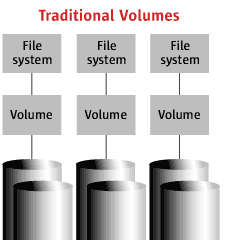
\includegraphics[width=5cm]{volumes_tradicionais.png}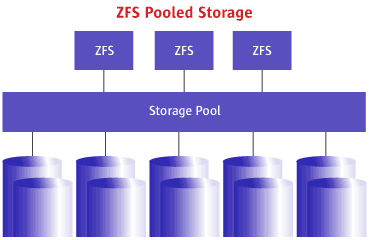
\includegraphics[width=7cm]{armazenamento_pooled_zfs.png}\\
	Voici les différentes unités de base de stockage de données :\\
	\begin{itemize}
		 \item Disques : entiers ou juste une partition
		 \item Fichiers dans un autre système de fichiers
		 \item Miroirs : 2 (ou plus) disques, partitions ou fichiers
		 \item Raid-z : plusieurs disques, variante de RAID-5\\
	\end{itemize}
	ZMirror est un miroir classique. Il utilise les mécanismes de checksum pour valider les lectures sur un composant et bascule sur le second s'il détecte une erreur puis corrige le composant défaillant (si possible). Le système Raid-z est similaire au procédé Raid 5. Il utilise les checksums (SHA-256 + fletcher) et repose sur le copy on write : supprime le "write-hole".
	\chapter*{Compression}
	Tout comme la déduplication, la compression est une technique qui permet d'économiser de l'espace de stockage. Chaque fichier est constitué d'une succession de millions de bits 0 ou 1. La compression permet de diminuer le nombre de bits que constitue un fichier en changeant la succession de bits de départ. Suivant l'algorithme de codage utilisé, le taux de compression peut différer. Les algorithmes d'encodage sont plus ou moins efficaces selon le type de fichier compressé.\\
 Il existe deux types de compression: la compression avec perte et sans perte. La compression sans perte signifie qu'après la décompression, le fichier sera identique au fichier compressé. C'est le plus souvent utilisé sur des documents, des fichiers exécutables ou des archives. Ces données étant principalement des caractères texte, ils ne peuvent pas être modifiés. Les formats de documentation tels que txt, doc ou pdf sont donc compressés sans perte.  Tant qu'à la compression avec perte, les fichiers décompressés ne seront pas exactement identiques au fichier original mais les informations seront sensiblement les mêmes. Les types de fichiers utilisés par cette compression sont les images, les sons et les vidéos. Cett technique se repose sur la limitation des sens de l'homme comme la vision et l'audition. L'homme ne pourra donc pas identifier les différences entre le fichier original et le fichier après décompressage. Les formats de fichiers jpeg, avi ou mp3 sont donc compressés avec pertes. \\
Pour chaque technique de compression, il existe plusieurs algorithmes de codage.\\
	\section{Compression sans perte}
		Parmi les algorithmes sans perte, il y a les algorithmes tels que Lempei-Ziv ou le codage RLE (Run-Length Encoding) qui consistent à remplacer des suites de bits utilisées plusieurs fois dans un même fichier. D'autres algorithmes comme l'algorithme de codage Huffman détermine les suites de bits et plus une suite est utilisée souvent, plus la suite qui la replacera sera courte. 
Voici les différents types de compression sans perte:
		\begin{itemize}
			\item L'algorithme Lempel-Ziv
			\begin{itemize}
				\item LZ77	
				\item LZ78
				\item LZO
			\end{itemize}
			\item L'algorithme RLE
			\item Codage par modélisation de contexte
			\begin{itemize}
				\item Prédiction par reconnaissance partielle (PPM)
				\item Pondération de contextes (CM)
			\end{itemize}
			\item L'algorithme de codage Huffman
		\end{itemize}
	\section{Compression avec pertes}
		La compression avec pertes s'utilisent donc sur des données perceptibles par l'homme comme les sons, les images ou les vidéos. Elles suppriment les données que l'homme ne perçoit pas ou quasiment pas. Ainsi pour le format JPEG 2000, la compression est de 1 bit/pixels au lieu de 24 bits/pixels. La compression avec pertes est une technique irréversible c'est à dire qu'il ne sera pas possible de retrouver le fichier original. Il existe trois grandes familles de compression avec pertes: la compression par prédiction, par transformation et la compression basée sur les récurrences fractales de motif.\\
 Voici les différents types de compression avec pertes:
		\begin{itemize}
			\item Compression par prédiction
			\item Compression par transformation
			\item La norme JPEG
			\item Compression par ondelette
			\item Compression basée sur les récurrences fractales de motif
		\end{itemize}
\end{document}
